
%%%%%%%%%%%%%%%%%%%%%%%%%%%%%%%%%%%%%%%%%%%%%%%%%%%%%%%%
\documentclass[12pt,a4paper]{article}% 文档格式
\usepackage{ctex,hyperref}% 输出汉字
\usepackage{times}% 英文使用Times New Roman
%%%%%%%%%%%%%%%%%%%%%%%%%%%%%%%%%%%%%%%%%%%%%%%%%%%%%%%%
\title{\fontsize{18pt}{27pt}\selectfont% 小四字号,1.5倍行距
	{\heiti% 黑体 
		Physics Homework}}% 题目
%%%%%%%%%%%%%%%%%%%%%%%%%%%%%%%%%%%%%%%%%%%%%%%%%%%%%%%%
\author{\fontsize{12pt}{18pt}\selectfont% 小四字号,1.5倍行距
	{\fangsong% 仿宋
		Haixuan Lin}\\% 标题栏脚注
	\fontsize{10.5pt}{15.75pt}\selectfont% 五号字号,1.5倍行距
	{\fangsong% 仿宋
		(Fudan University department of physics
		)}}% 作者单位,“~”表示空格
%%%%%%%%%%%%%%%%%%%%%%%%%%%%%%%%%%%%%%%%%%%%%%%%%%%%%%%%
\date{}% 日期(这里避免生成日期)
%%%%%%%%%%%%%%%%%%%%%%%%%%%%%%%%%%%%%%%%%%%%%%%%%%%%%%%%
\usepackage{amsmath,amsfonts,amssymb}% 为公式输入创造条件的宏包
%%%%%%%%%%%%%%%%%%%%%%%%%%%%%%%%%%%%%%%%%%%%%%%%%%%%%%%%
\usepackage{graphicx}% 图片插入宏包
\usepackage{subfigure}% 并排子图
\usepackage{float}% 浮动环境,用于调整图片位置
\usepackage[export]{adjustbox}% 防止过宽的图片
\usepackage{pdfpages}
%%%%%%%%%%%%%%%%%%%%%%%%%%%%%%%%%%%%%%%%%%%%%%%%%%%%%%%%
\usepackage{bibentry}
\usepackage{natbib}% 以上2个为参考文献宏包
%%%%%%%%%%%%%%%%%%%%%%%%%%%%%%%%%%%%%%%%%%%%%%%%%%%%%%%%
\usepackage{abstract}% 两栏文档,一栏摘要及关键字宏包
\renewcommand{\abstracttextfont}{\fangsong}% 摘要内容字体为仿宋
\renewcommand{\abstractname}{\textbf{摘\quad 要}}% 更改摘要二字的样式
%%%%%%%%%%%%%%%%%%%%%%%%%%%%%%%%%%%%%%%%%%%%%%%%%%%%%%%%
\usepackage{xcolor}% 字体颜色宏包
\newcommand{\red}[1]{\textcolor[rgb]{1.00,0.00,0.00}{#1}}
\newcommand{\blue}[1]{\textcolor[rgb]{0.00,0.00,1.00}{#1}}
\newcommand{\green}[1]{\textcolor[rgb]{0.00,1.00,0.00}{#1}}
\newcommand{\darkblue}[1]
{\textcolor[rgb]{0.00,0.00,0.50}{#1}}
\newcommand{\darkgreen}[1]
{\textcolor[rgb]{0.00,0.37,0.00}{#1}}
\newcommand{\darkred}[1]{\textcolor[rgb]{0.60,0.00,0.00}{#1}}
\newcommand{\brown}[1]{\textcolor[rgb]{0.50,0.30,0.00}{#1}}
\newcommand{\purple}[1]{\textcolor[rgb]{0.50,0.00,0.50}{#1}}% 为使用方便而编辑的新指令
\renewcommand{\d}{\mathrm{d}}
%%%%%%%%%%%%%%%%%%%%%%%%%%%%%%%%%%%%%%%%%%%%%%%%%%%%%%%%
\usepackage{url}% 超链接
\usepackage{bm}% 加粗部分公式
\usepackage{multirow}
\usepackage{booktabs}
\usepackage{epstopdf}
\usepackage{epsfig}
\usepackage{longtable}% 长表格
\usepackage{supertabular}% 跨页表格
\usepackage{algorithm}
\usepackage{algorithmic}
\usepackage{changepage}% 换页
%%%%%%%%%%%%%%%%%%%%%%%%%%%%%%%%%%%%%%%%%%%%%%%%%%%%%%%%
\usepackage{enumerate}% 短编号
\usepackage{caption}% 设置标题
\captionsetup[figure]{name=\fontsize{10pt}{15pt}\selectfont Figure}% 设置图片编号头
\captionsetup[table]{name=\fontsize{10pt}{15pt}\selectfont Table}% 设置表格编号头
%%%%%%%%%%%%%%%%%%%%%%%%%%%%%%%%%%%%%%%%%%%%%%%%%%%%%%%%
%\usepackage{indentfirst}% 中文首行缩进
\usepackage[left=2.50cm,right=2.50cm,top=2.80cm,bottom=2.50cm]{geometry}% 页边距设置
\renewcommand{\baselinestretch}{1.5}% 定义行间距(1.5)
%%%%%%%%%%%%%%%%%%%%%%%%%%%%%%%%%%%%%%%%%%%%%%%%%%%%%%%%
\usepackage{fancyhdr} %设置全文页眉、页脚的格式
\pagestyle{fancy}
\hypersetup{colorlinks=true,linkcolor=black}% 去除引用红框,改变颜色
%%%%%%%%%%%%%%%%%%%%%%%%%%%%%%%%%%%%%%%%%%%%%%%%%%%%%%%%
\usepackage{caption}%标题取消自动figure
\usepackage{multicol}
\usepackage{cuted}
%%%%%%%%%%%%%%%%%%%%%%%%%%%%%%%%%%%%%%%%%%%%%%%%%%%%%%%%
\newcommand{\nonumbersection}[1]{
	\section*{#1}
	\addcontentsline{toc}{section}{#1}
}
\newcommand{\nonumbersubsection}[1]{
	\subsection*{#1}
	\addcontentsline{toc}{subsection}{#1}
}
%%%%%%%%%%%%%%%%%%%%%%%%%%%%%%%%%%%%%%%%%%%%%%%%%%%%%%%%
\begin{document}% 以下为正文内容
	\maketitle% 产生标题,没有它无法显示标题
	%%%%%%%%%%%%%%%%%%%%%%%%%%%%%%%%%%%%%%%%%%%%%%%%%%%%%%%%
	\lhead{}% 页眉左边设为空
	\chead{}% 页眉中间设为空
	\rhead{}% 页眉右边设为空
	\lfoot{}% 页脚左边设为空
	\cfoot{\thepage}% 页脚中间显示页码
	\rfoot{}% 页脚右边设为空
	%%%%%%%%%%%%%%%%%%%%%%%%%%%%%%%%%%%%%%%%%%%%%%%%%%%%%%%%
	
	
	\begin{center}% 居中处理
		{\textbf{Abstract}}% 英文摘要
	\end{center}
	\begin{adjustwidth}{1.06cm}{1.06cm}% 英文摘要内容
		\hspace{1.5em}In order to improve my computer and English skills, please allow me to complete this physics homework in English context with \LaTeX, so as to improve my professional level. Sorry for the inconvenience!
	\end{adjustwidth}
	
	\newpage% 从新的一页继续
	
	\renewcommand{\contentsname}{Contents}
	\tableofcontents
	\newpage
	
	\nonumbersection{Question 7-5}
	 \begin{figure}[h]
	 	\centering
	 	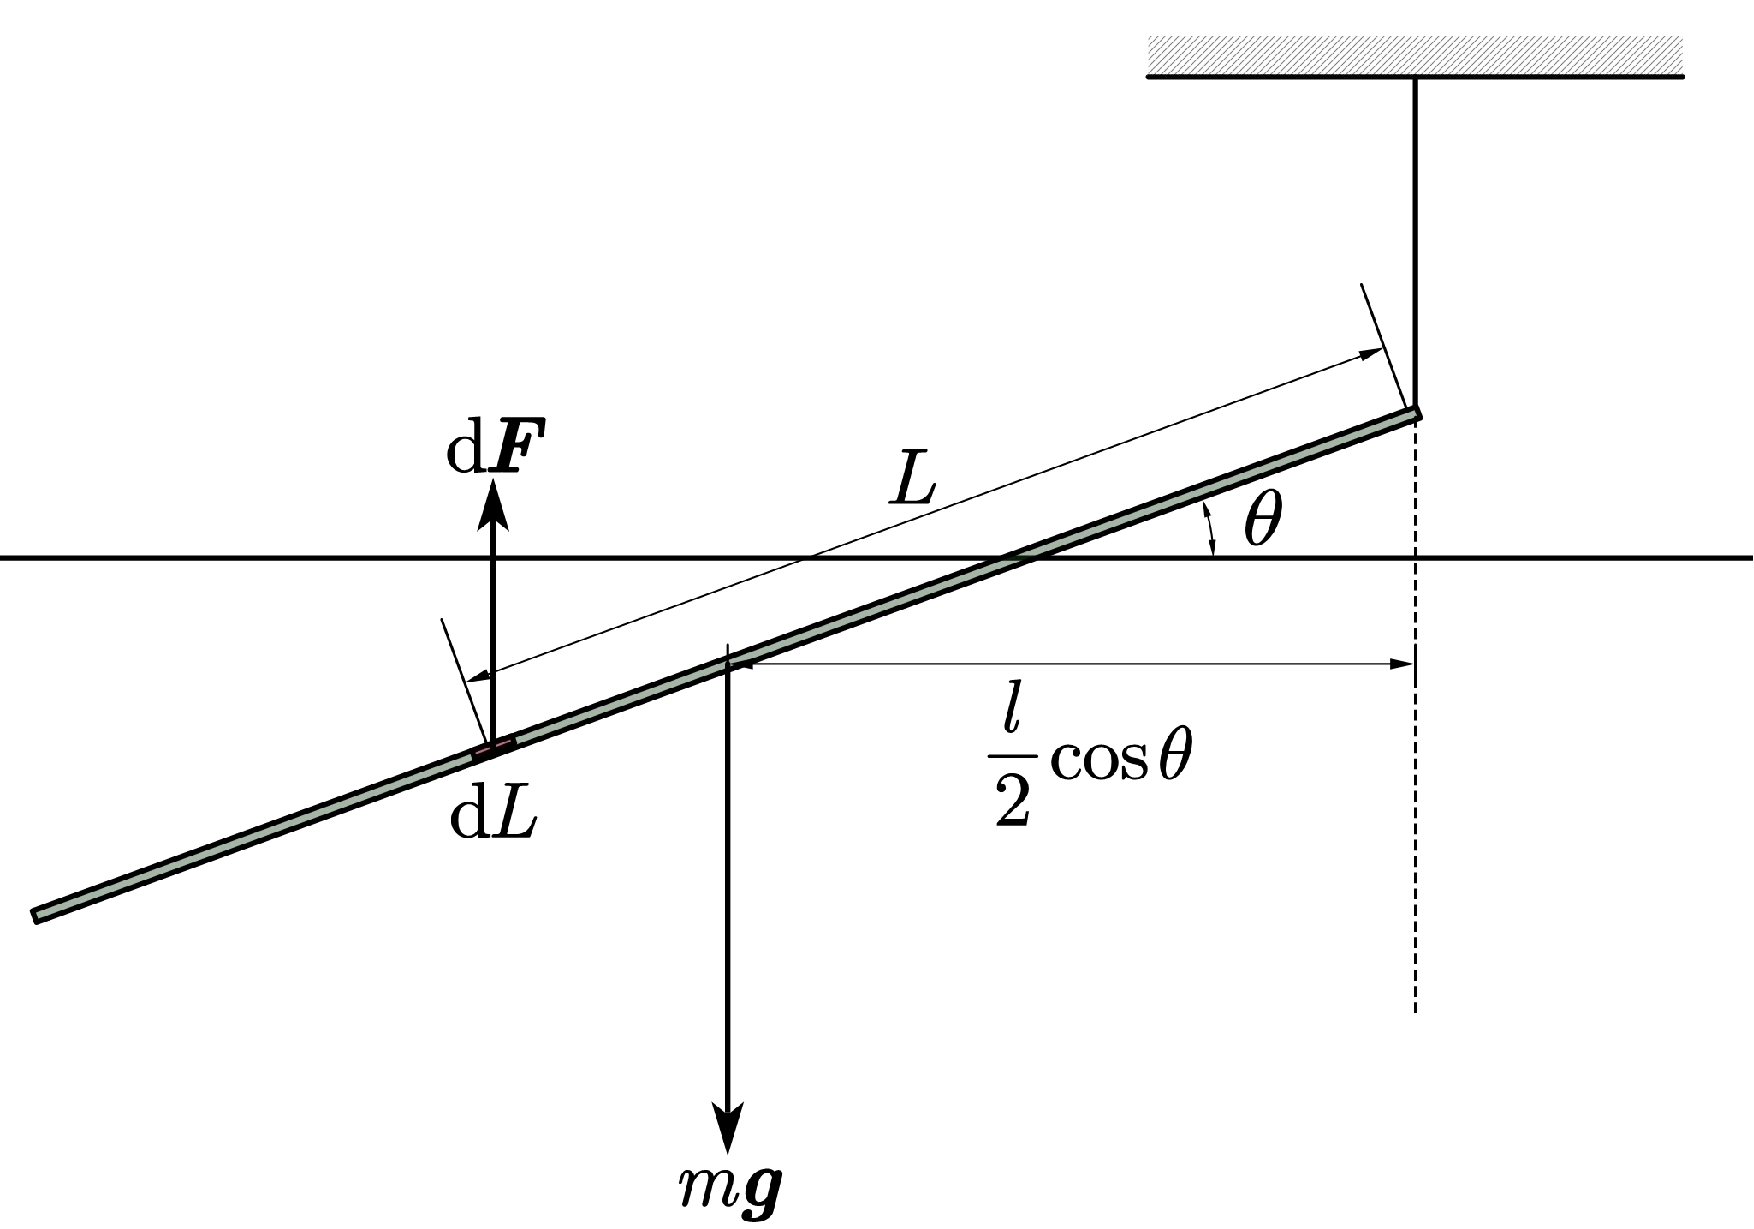
\includegraphics[width=0.7\linewidth]{C:/Users/Administrator/Desktop/VScode/LaTeX/Early Pic/7-5}
	 	\caption*{}
	 	\label{fig:7-5}
	 \end{figure}
	 \nonumbersubsection{(1)}
	\noindent Let's take a tiny element to analyse. The force and moment can get with point where rod and rope tied together as reference point.
	\begin{equation}
		\mathrm{d}F=\rho_0g\mathrm{d}V=\rho_0gS\d L
	\end{equation}
	\begin{equation}
		\d M_F=\d FL\cos\theta =\rho_0gS\cos\theta L\d L
	\end{equation}
	And we can get the moment of $\boldsymbol{F}$ by integrating.
	\begin{equation}
		M_F=\int \d M_F=\left.\frac{1}{2}\rho_0gS\cos\theta L^2\right|_{d\csc\theta}^l=\frac{1}{2}\rho_0gS\cos\theta(l^2-d^2\csc^2\theta)
	\end{equation}
	And the moment of gravity is easy to get.
	\begin{equation}
		M_G=mg\frac{l}{2}\cos\theta=\rho glS\frac{l}{2}\cos\theta
	\end{equation}
	And the torque equilibrium equation will get.
	\begin{equation}
		M_G=M_F
	\end{equation}
	The solution is below.
	$$
	\theta=\arcsin \frac{d}{l\sqrt{1-\cfrac{\rho}{\rho_0}}}
	$$
	\nonumbersubsection{(2)}
	\noindent We can get the $\boldsymbol{F}$ by integrating.
	\begin{equation}
		F=\left.\int \d F=\rho_0gSL\right|_{d\csc\theta}^l=\rho_0gS\left(l-d\csc\theta\right)
	\end{equation}
	According to the force balance, we can get $\boldsymbol{F}_\mathrm{T}$.
	$$
	F_\mathrm{T}=mg-F=\left(\rho-\rho_0+\rho_0\sqrt{1-\cfrac{\rho}{\rho_0}}\right)lSg
	$$
	\nonumbersection{Question 7-9}
	\nonumbersubsection{(1)}
	\noindent Equation of continuity is below.
	\begin{equation}
		Sv_A=Sv_B=Sv_C
	\end{equation}
	According to Torricelli's theorem.
	\begin{equation}
		v_B=\sqrt{2g\left( h_A-h_B\right) }
	\end{equation}
	Compare point A with liquid level of the same height, according to the Bernoulli's equation,
	\begin{equation}
		p_0=p_A+\frac{1}{2}\rho v_A^2
	\end{equation}
	The same method.
	\begin{equation}
		p_0=p_C+\frac{1}{2}\rho v_C^2+\rho g(h_C-h_A)
	\end{equation}
	So we solve it.
	\begin{align*}
		p_A&=p_0-\rho g(h_A-h_B)\approx0.915\times10^5\ \mathrm{Pa}
		\\
		p_B&=p_0\approx1.013\times10^5\ \mathrm{Pa}
		\\
		p_C&=p_0-\rho g(h_C-h_B)\approx0.866\times10^5\ \mathrm{Pa}
	\end{align*}
	\nonumbersubsection{(2)}
	\noindent	According to the definition of fluid flow.
	\begin{equation}
		Q=Sv
	\end{equation}
	So we have.
	$$
	Q=Sv\approx3.10\times10^{-3}\ \mathrm{m^3/s}
	$$
	\nonumbersubsection{(3)}
	\noindent The critical condition requires $p_C=0$, so.
	\begin{equation}
		p_0=\rho gh_{C_\mathrm{max}}+\frac{1}{2}\rho v_C^2
	\end{equation}
	Here we consider $p_0=1.00\times 10^5\ \mathrm{Pa}$. The solution is that.
	$$
	h_{C_\mathrm{max}}=\frac{p_0-\rho g\left( h_A-h_B \right)}{\rho g}\approx9.20\ \mathrm{m}
	$$
	\nonumbersection{Question 7-10}
	\noindent Examine the fluid in the pipe. According to the equation of continuity.
	\begin{equation}
		S_Av_A=S_Bv_B=Q
	\end{equation}
	According to Bernoulli's equation.
	\begin{equation}
		p_A+\frac{1}{2}\rho v_{A}^{2}=p_B+\frac{1}{2}\rho v_{B}^{2}
	\end{equation}
	And the pipe B is conect with air.
	\begin{equation}
		p_B=p_0
	\end{equation}
	At the same time, the pipe A and the tiny pipe below form a communication device.
	\begin{equation}
		p_A+\rho gh=p_0
	\end{equation}
	So.
	$$
	h=\frac{Q^2}{2g}\left(\frac{1}{S_A^2}-\frac{1}{S_B^2} \right) 
	$$
	\nonumbersection{Questuon 7-11}
	\noindent Static pressure changes to dynamic pressure when the fluid passes through point B.
	\begin{equation}
		\frac{1}{2}\rho \left( v_{B}^{2}-v_{A}^{2} \right) =\rho 'gh
	\end{equation}
	And we have the equation of continuity.
	\begin{equation}
		S_Av_A=S_Bv_B
	\end{equation}
	So.
	$$
	v_A=\sqrt{\frac{2\rho'gh}{\rho\left( \cfrac{S_A^2}{S_B^2}-1\right) }}\approx0.56\ \mathrm{m/s}
	$$
	\nonumbersection{Question 7-12}
	\noindent According to Bernoulli's equation.
	\begin{equation}
		p_0+\Delta p=p_0+\rho gh+\frac{1}{2}\rho v^2
	\end{equation}
	So.
	$$
	\Delta p=\rho gh+\frac{1}{2}\rho v^2\approx6.025\times10^3\ \mathrm{Pa}
	$$
	\nonumbersection{Question 7-13}
	\nonumbersubsection{(1)}
	\noindent  It is easy to know that the outflow velocity of water is below.
	\begin{equation}
		v_0=\sqrt{2gH}
	\end{equation}
	So.
	$$
	Q=\pi \left(\frac{d}{2} \right)^2v_0 =\frac{1}{4}\pi d^2\sqrt{2gH}
	$$
	\nonumbersubsection{(2)}
	According to the Bernoulli's equation.
	\begin{equation}
		p_{\mathrm{up}}+\frac{1}{2}\rho v_{0}^{2}+\rho gh=p_{\mathrm{down}}+\frac{1}{2}\rho v_{\mathrm{down}}^{2}
	\end{equation}
	According to the equation of continuity.
	\begin{equation}
		\pi \left( \frac{D}{2} \right) ^2v_{\mathrm{down}}=Q
	\end{equation}
	And.
	\begin{equation}
		p_\mathrm{up}=p_0
	\end{equation}
	So.
	$$
	p_{\mathrm{down}}=p_0+\rho gh+\rho gH\left( 1-\frac{d^4}{D^4}\right) 
	$$
	\nonumbersection{Question 7-14}
	\nonumbersubsection{(1)}
	\noindent According to the communicator principle.
	$$
	h_1=h_A
	$$
	\nonumbersubsection{(2)}
	\noindent The static pressure at B after discharge becomes $p_0$. According to the communicator principle.
	$$
	h_2=h_C
	$$
	\nonumbersection{Question 7-17}
	\noindent According to the Bernoulli's equation and continuity equation.
	\begin{equation}
		v=\sqrt{2gH}
	\end{equation}
	\begin{equation}
		Sv=\pi\left(\frac{R}{h}H \right)^2\frac{-\d H}{\d t} 
	\end{equation}
	Here we ignore the velocity of the free liquid surface. And.
	\begin{equation}
		-H^{\frac{3}{2}}\mathrm{d}H=\frac{Sh^2}{\pi ^2R^2}\sqrt{2g}\mathrm{d}t
	\end{equation}
	 $$
	 t=\frac{-\pi ^2R^2}{Sh^2\sqrt{2g}}\int_h^{\frac{1}{2}h}{H^{\frac{3}{2}}\mathrm{d}H}
	 =\frac{\pi^2R^2}{20S}\sqrt{\frac{h}{g}}(4\sqrt{2}-1)
	 $$
	 \nonumbersection{Question 7-23}
	 \begin{figure}[h]
	 	\centering
	 	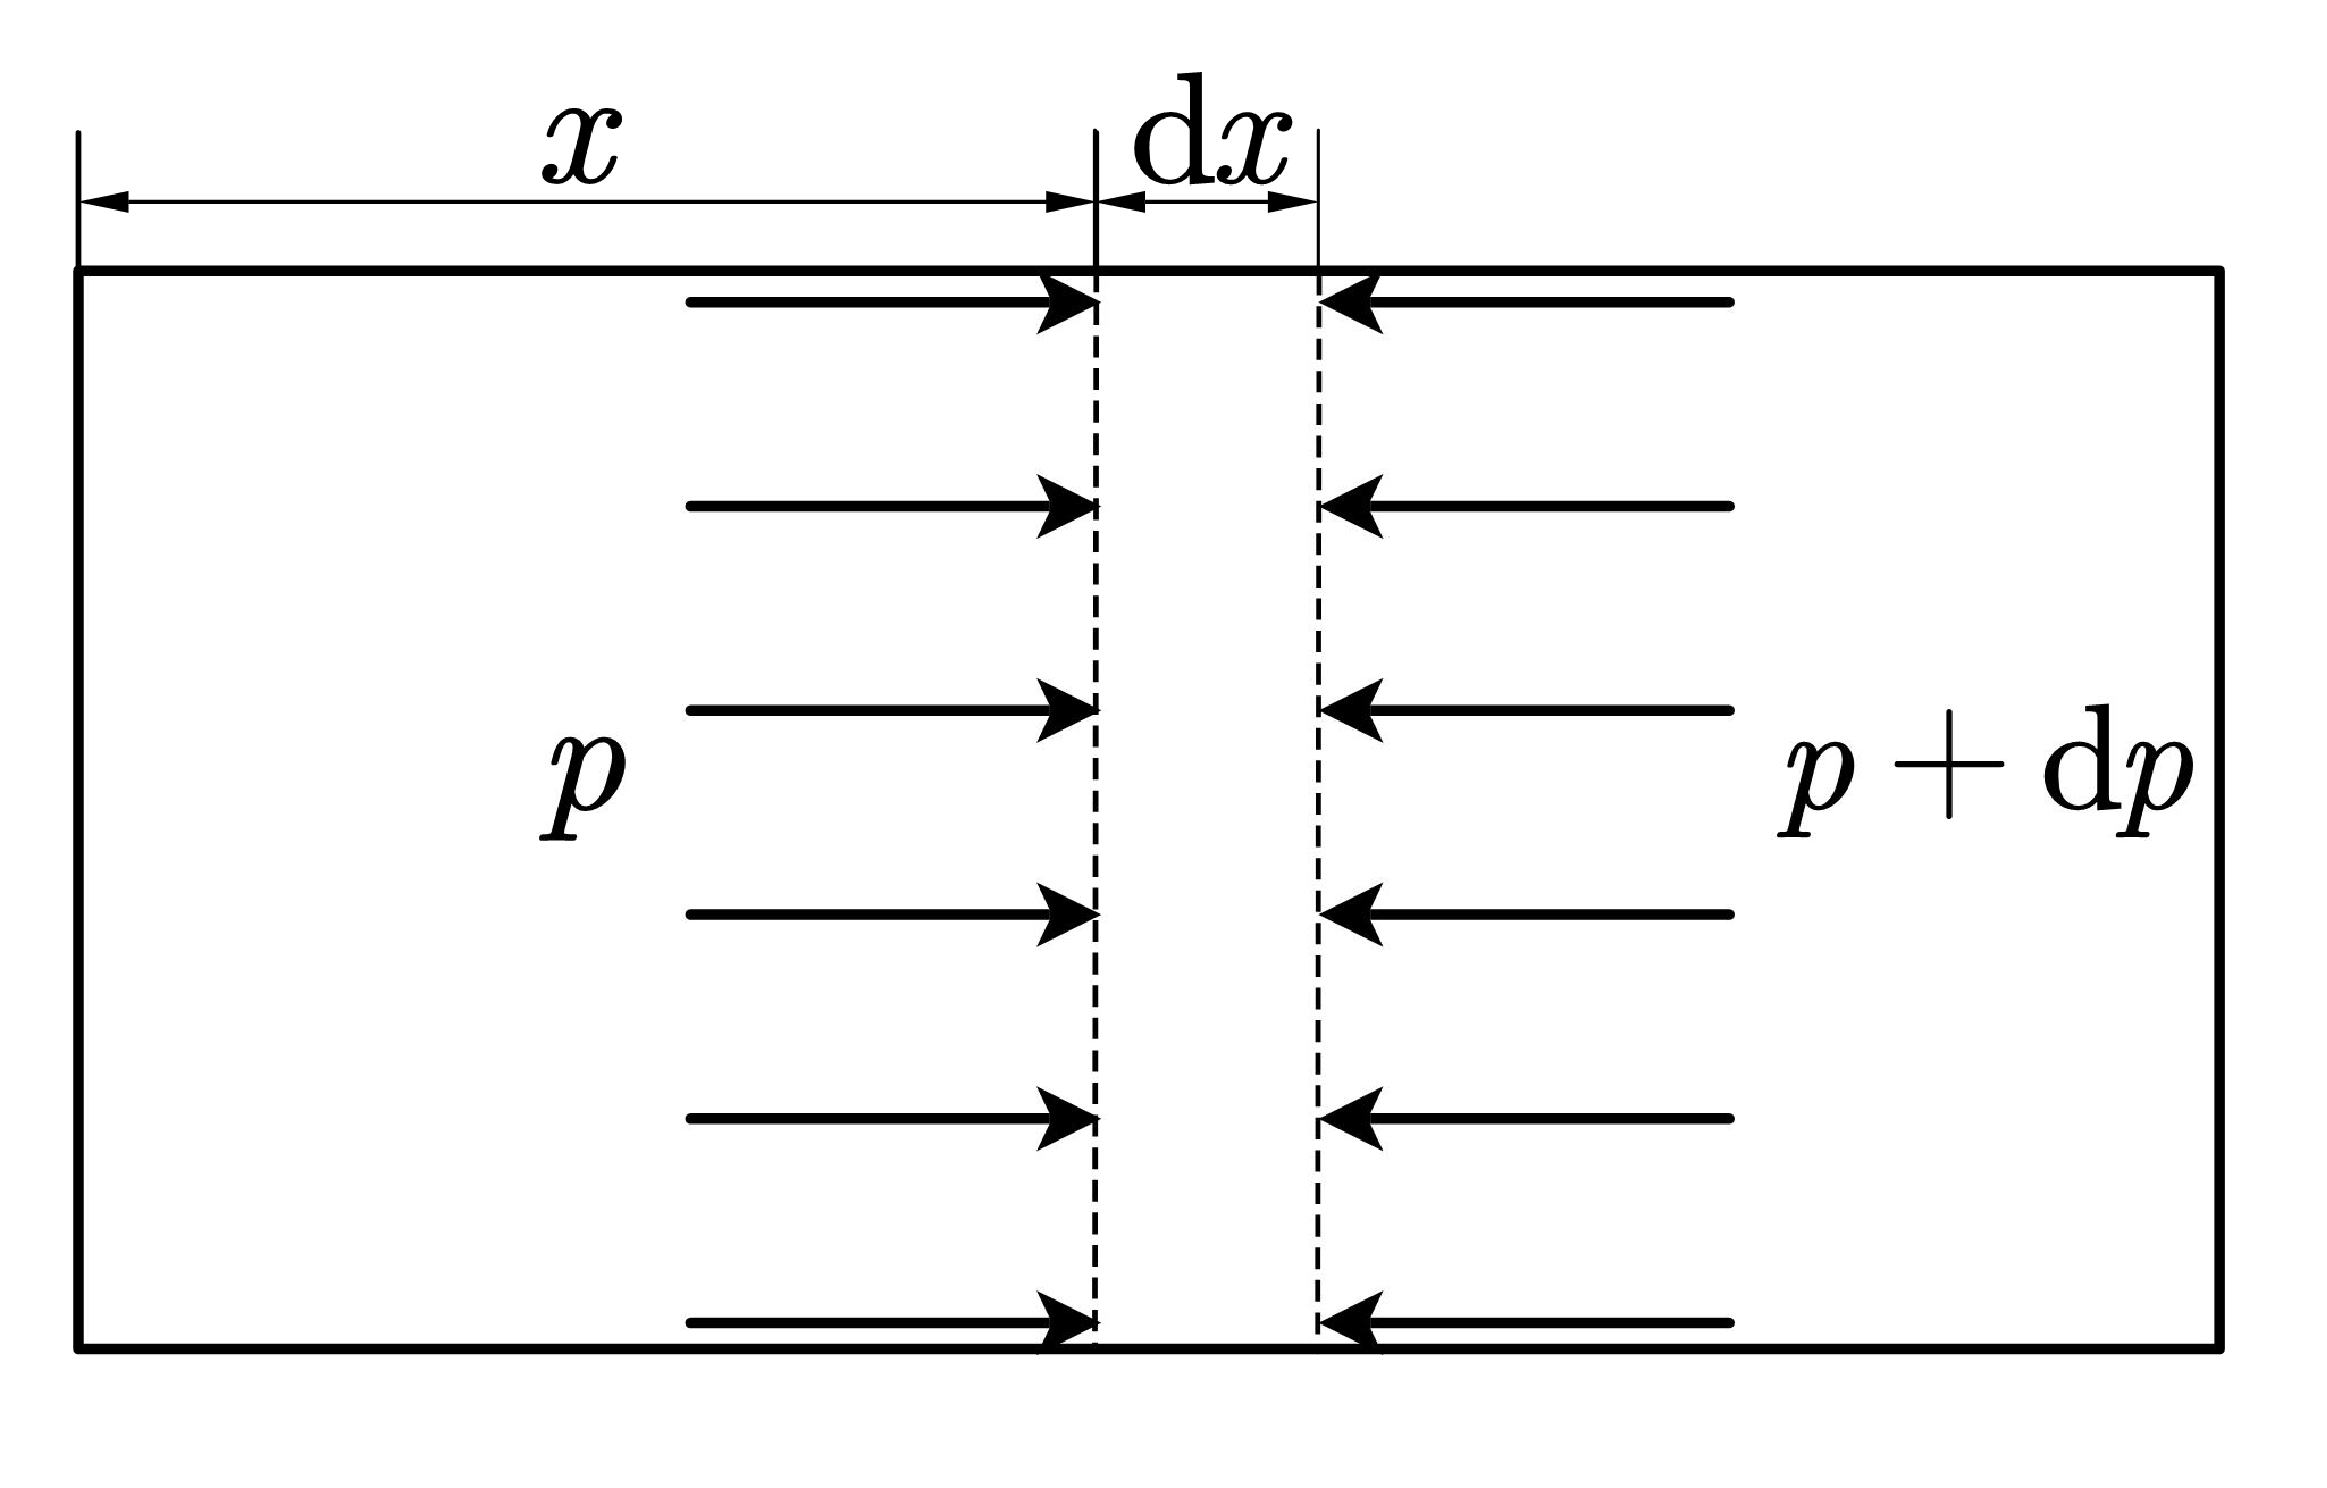
\includegraphics[width=0.7\linewidth]{C:/Users/Administrator/Desktop/VScode/LaTeX/Early Pic/7-23}
	 	\caption*{}
	 	\label{fig:7-23}
	 	\end{figure}
	 \noindent Because of centrifugal force, air molecules have a tendency to move outward in a radial direction. It is obtained by air thin layer study which length is $\d x$ and force analysis.
	 \begin{equation}
	 	\d pS=S\d x\rho(x)\omega^2x
	 \end{equation}
	 The ideal gas equation of state can be derived from the relationship between density and pressure
	 \begin{equation}
	 	pV=nRT=\frac{m}{M_\mathrm{mol}}RT\Longrightarrow pM_\mathrm{mol}=\frac{m}{V}RT=\rho RT
	 \end{equation}
	 As a result.
	 \begin{equation}
	 	\frac{\mathrm{d}p}{p}=\frac{\rho _0\omega ^2}{p_0}x\mathrm{d}x
	 \end{equation}
	 The solution is as below.
	 \begin{equation}
	 	p\left( x \right) =p\left( x=0 \right) \mathrm{e}^{\dfrac{\rho _0\omega ^2}{2p_0}\displaystyle{x^2} }
	 \end{equation}
	 And we know that the $\omega$ is very very small. So we can do Tailor expand.
	 \begin{equation}
	 	p(x)\sim p(x=0)\left( \cfrac{\rho _0\omega ^2}{2p_0}x^2+1\right) 
	 \end{equation}
	 By the law of conservation of mass.
	 \begin{equation}
	 	\int_{0}^{L}p(x)\d x=\int_{0}^{L}p_0\d x
	 \end{equation}
	 And.
	 \begin{equation}
	 	\int_{0}^{L}p(x)\d x\sim\int_{0}^{L}p(x=0)\left( \cfrac{\rho _0\omega ^2}{2p_0}x^2+1\right) \d x=p_0L
	 \end{equation}
	 We get.
	 \begin{equation}
	 	p(x=0)=\dfrac{p_0}{\dfrac{\rho _0\omega ^2}{6p_0}L^2+1}\sim p_0\left( 1-\frac{\rho _0\omega ^2}{6p_0}L^2\right) 
	 \end{equation}
	 According to the communicator principle.
	 \begin{equation}
	 	p_0-p(x=0)=\rho gh
	 \end{equation}
	 We solve this problem.
	 $$
	 h=\frac{L^2\omega^2\rho_0}{6\rho g}
	 $$
\end{document}